\documentclass[a4paper]{article}
\usepackage[letterpaper, margin=1in]{geometry} % page format
\usepackage{listings} % this package is for including code
\usepackage{graphicx} % this package is for including figures
\usepackage{amsmath}  % this package is for math and matrices
\usepackage{amsfonts} % this package is for math fonts
\usepackage{tikz} % for drawings
\usepackage{hyperref} % for urls

\title{Homework2}
\author{Morgan Baker}
\date{9/27/16}

\begin{document}
\lstset{language=Python}

\maketitle

\section{Question 2.1}
$\varepsilon(M,N,\delta)\leq\sqrt{\frac{1}{2N}ln(\frac{2M}{\delta})}$\\
I used this equation and just plugged in the numbers. The function $\varepsilon$ was set to .05, $\delta$ was set to .03, and depending on the part of the question, M could be set to either 1, 100, or 10000.

\subsection{Answer to Part A}
In part A, M is equal to 1.\\
$.05\leq\sqrt{\frac{1}{2N}ln(\frac{2M}{.03})}$\\
$.05\leq\sqrt{\frac{1}{2N}ln(\frac{2}{.03})}$\\
$.05\leq\sqrt{\frac{1}{2N}ln(66.66666)}$\\
$.0025\leq\frac{1}{2N}ln(66.66666)$\\
$.005N\leq4.2$\\
$N\leq840$

\subsection{Answer to Part B}
In part B, M is equal to 100.\\
$.05\leq\sqrt{\frac{1}{2N}ln(\frac{2M}{.03})}$\\
$.05\leq\sqrt{\frac{1}{2N}ln(\frac{200}{.03})}$\\
$.05\leq\sqrt{\frac{1}{2N}ln(6666.666)}$\\
$.0025\leq\frac{1}{2N}ln(6666.666)$\\
$.005N\leq8.8$\\
$N\leq1760$

\subsection{Answer to Part C}
In part C, M is equal to 10000.\\
$.05\leq\sqrt{\frac{1}{2N}ln(\frac{2M}{.03})}$\\
$.05\leq\sqrt{\frac{1}{2N}ln(\frac{20000}{.03})}$\\
$.05\leq\sqrt{\frac{1}{2N}ln(666666.666)}$\\
$.0025\leq\frac{1}{2N}ln(666666.666)$\\
$.005N\leq13.41$\\
$N\leq2682$

\section{Question 2.11}
$E_{out}(g)\leq E_{in}(g)+\sqrt{\frac{8}{N}ln(\frac{4m_\mathcal{H}(2N)}{\delta})}$\\
Again, another equation to start plugging and chugging. In this case, $\delta$ is .1, and $m_\mathcal{H}$ is equal to 2n + 1.
\subsection{Part 1}
Part 1 asks us to solve the equation when N = 100.
$E_{out}(g)\leq E_{in}(g)+\sqrt{\frac{8}{N}ln(\frac{4(2N+1)}{.1})}$\\
$E_{out}(g)\leq E_{in}(g)+\sqrt{\frac{8}{100}ln(\frac{4(2(100)+1)}{.1})}$\\
$E_{out}(g)\leq E_{in}(g)+\sqrt{.08ln(8040)}$\\
$E_{out}(g)\leq E_{in}(g)+\sqrt{.08*9}$\\
$E_{out}(g)\leq E_{in}(g)+\sqrt{.72}$\\
$E_{out}(g)\leq E_{in}(g)+.84$
\subsection{Part 2}
Part 1 asks us to solve the equation when N = 10000.
$E_{out}(g)\leq E_{in}(g)+\sqrt{\frac{8}{N}ln(\frac{4(2N+1)}{.1})}$\\
$E_{out}(g)\leq E_{in}(g)+\sqrt{\frac{8}{10000}ln(\frac{4(2(10000)+1)}{.1})}$\\
$E_{out}(g)\leq E_{in}(g)+\sqrt{.0008ln(800040)}$\\
$E_{out}(g)\leq E_{in}(g)+\sqrt{.08*13.6}$\\
$E_{out}(g)\leq E_{in}(g)+\sqrt{.012}$\\
$E_{out}(g)\leq E_{in}(g)+.1$\\

\section{Question 2.12}
$N\geq\frac{8}{\varepsilon^2}ln(\frac{4((2N)^{10}+1)}{\delta})$\\
While looking in the book, the advice given for figuring out these kinds of equations was to throw something in for N and re-iterate the function to find where both sides are equal. To make it easeir on myself to enter in values for the function, I simplified it, shown below.
$N\geq\frac{8}{0.05^2}ln(\frac{4((2N)^{10}+1)}{0.05})$\\
$N\geq\frac{8}{0.025}(ln(4(1024N^{10}+1))-ln(0.05))$\\
$N\geq3200(ln(4096)+10ln(N)+ln(4)-ln(0.05))$\\
$N\geq3200(ln(\frac{4096(4)}{0.05})+10ln(N))$\\
$N\geq3200(12.7+10ln(N))$\\
$N\geq40639+32000ln(N)$\\
At this point, I thought the equation was simplified enough to where I would only need to do one natural logarithm per iteration. So, it began with 1000.\\
$N\geq40639+32000ln(1000)$\\
$N\geq40639+221048.168$\\
Now, because 261687 is definitely more than 1000, I plugged that number in for the new N.\\
$N\geq40639+32000ln(261687)$\\
$N\geq40639+393888.696$\\
Again, becuase 393888 is larger than 261687, we throw it back in there.\\
$N\geq40639+32000ln(393888)$\\
$N\geq40639+412282.300$\\
This equals out to about 452921. I finally decided to throw the function into a graphing calculator and got 457728, which was suprisingly close to what I got after four iterations. 

\section{Question 3.1}
This was a confusing one. The first part of the question was to plot a group of points that made two semicircles. Luckily, Professor Rivas uploaded some code to help us out. Using the Perceptron.py class from Rivas, now renamed SemiCirclePerceptron.py just for clarity, I was able to run the program and get the figure here (\ref{fig:figure_3}). The second part of the question is to use linear regression to figure out a middle ground. Linear regreesion is, put simply, finding a middle ground between the points of data in a dataset. The second image here (\ref{fig:figure_1}) shows this being done. While not completely separate, it still looks pretty. Most of the points that are missed are near the edges of the semicircles.
\begin{figure}
  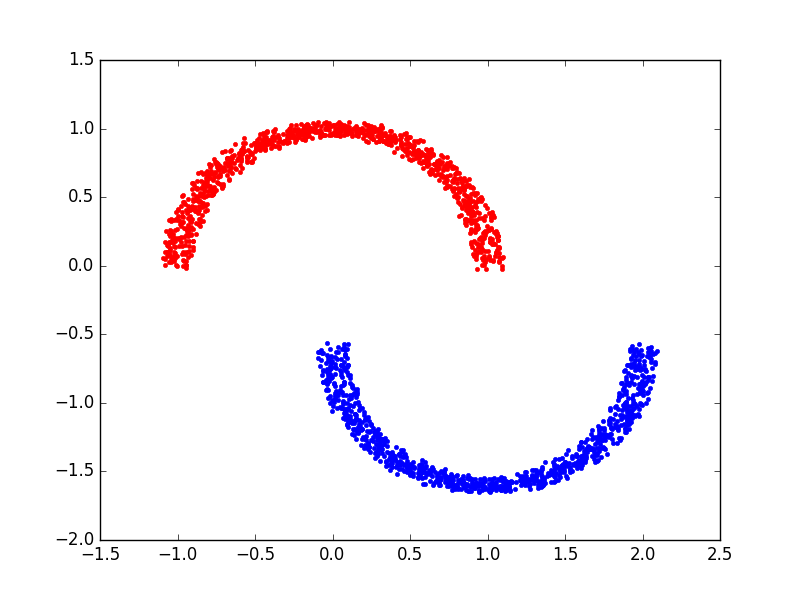
\includegraphics[width=9cm,height=9cm]{figure_3.png}
  \caption{The plot of 2000 points using the code provided by Professor Rivas.}
  \label{fig:figure_3}
\end{figure}
\begin{figure}
  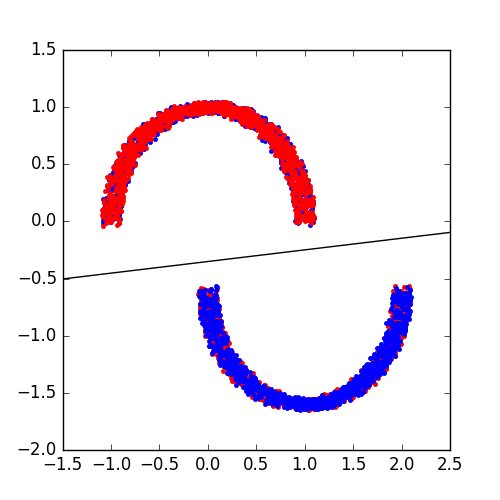
\includegraphics[width=9cm,height=9cm]{figure_1.png}
  \caption{The plot of 2000 points using linear regression.}
  \label{fig:figure_1}
\end{figure}

\end{document}